\chapter{JTAG Overview}
This chapter gives an overview of the JTAG  and partitioning of the JTAG. It contains the following sections:
\begin{itemize}
    \item \hyperref[sec:system-overview]{System Overview}
    \item \hyperref[sec:bst-arhitecture]{Boundary Scan Testing Architecture}
    \item \hyperref[sec:jtag-partitioning]{JTAG Partitioning}
\end{itemize}
\newpage

\section{System Overview}
\label{sec:system-overview}
In JTAG, testing and debugging is carried through Test Access Port (TAP) which contains four mandatory pins (TDI, TMS, TCK, TDO) and an optional pin for asynchronous reset (TRST). A  TAP/JTAG controller is a module that controls and coordinates the operations of the entire test architecture.

The Figure \ref{fig:zic_partitioning} shows the conceptual view of top level JTAG design.

\vspace{1cm}
\begin{figure}[H]
    \centering
    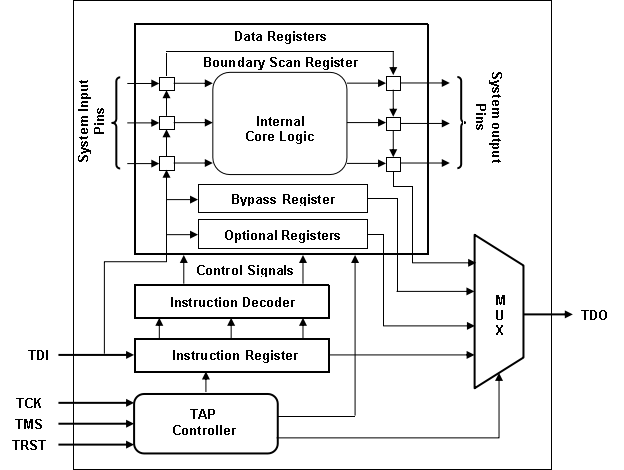
\includegraphics[width = 15cm]{images/jtag_block_diagram.png}
    \vspace{1cm}
    \caption{ZIC Partitioning}
    \label{fig:zic_partitioning}
\end{figure}
\vspace{1cm}

The sequence of operation is as follows

\begin{enumerate}
    \item The TAP controller receives TCK and interprets the signals on TMS. The TAP controller generates clock or control signals or both as required for the instruction and test data registers and for other parts of the design.
    \item  The TAP controller controls the operation (normal, shift, capture, update) while instruction decoder provides the context of the operation (i.e., to which register and associated test logic the action applies).
    \item The instruction register allows the instruction to be shifted into the design. The instruction is used to select the test to be performed or the test data register to be accessed or both.
    \item The instruction register is never undefined and always selects a single test data register to connect between TDI and TDO.
    \item The group of test data registers shall include a bypass and a boundary-scan register. It also may include any of the optional standard test data registers: the device identification, initialization data, initialization status, TMP control, and reset selection registers; and further optional design specific test data registers. 
    \item A circuit controlled by instruction decoder selects the test data register to drive the output TDO.
\end{enumerate}

\section{Boundary Scan Testing Architecture}
\label{sec:bst-arhitecture}

Boundary scan is a method for testing interconnects (wire lines) on printed circuit boards or sub-blocks inside an integrated circuit. 

\vspace{1cm}
\begin{figure}[H]
    \centering
    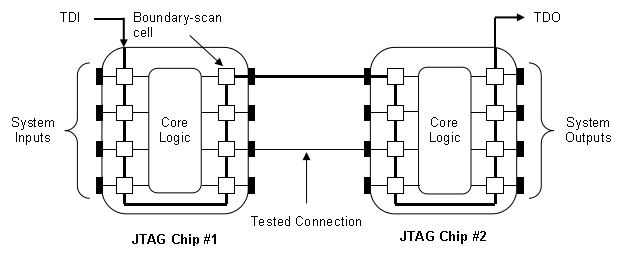
\includegraphics[width = 14cm]{images/boundary_scan_test.png}
    \vspace{1cm}
    \caption{Boundary Scan Test}
    \label{fig:bst}
\end{figure}
\vspace{1cm}

Boundary scan is also widely used for 
\begin{enumerate}
    \item Debugging - watch integrated circuit pin states
    \item Board-level test and diagnosis
    \item Test on-board interconnect among chips
    \item Test on-chip system logic
\end{enumerate}

\section{JTAG Partitioning}
\label{sec:jtag-partitioning}

 The JTAG architecture is partitioned into the following functional blocks
\begin{enumerate}
    \item \hyperref[chap:TAP]{Test Access Port (TAP)}
    \item \hyperref[chap:instruction-reg]{Instruction Register}
    \item \hyperref[chap:data-reg]{Test Data Registers}
\end{enumerate}

The instruction and test data registers shall be separate shift-register based paths that are connected in parallel and have a common serial data input and a common serial data output connected to the TAP TDI and TDO signals, respectively. 

The selection between the alternative instruction and test data register paths between TDI and TDO shall be made under the control of the TAP controller.